\documentclass[border=8pt]{standalone}
\usepackage{tikz}
\usetikzlibrary{arrows.meta,positioning,calc,fit}
\begin{document}
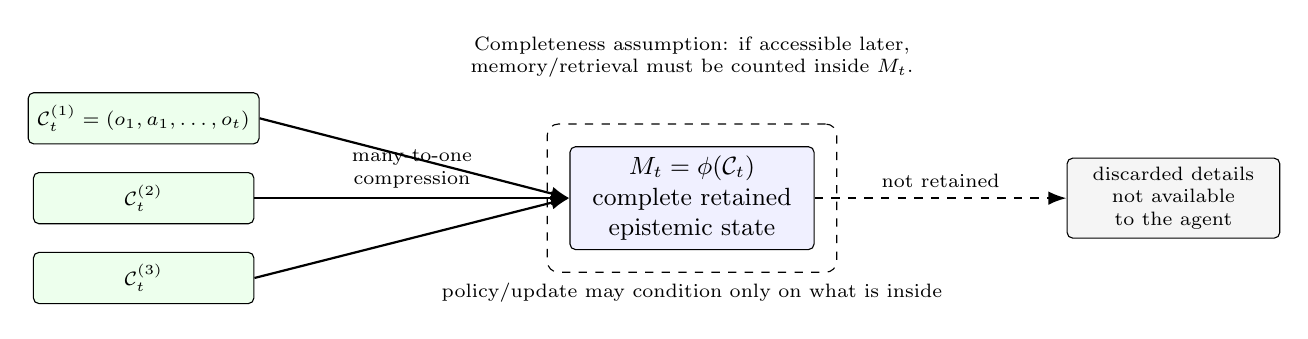
\begin{tikzpicture}[
  hist/.style={draw, rounded corners=2pt, align=center, minimum width=2.8cm, minimum height=0.65cm, font=\scriptsize, fill=green!7},
  model/.style={draw, rounded corners=2pt, align=center, minimum width=3.1cm, minimum height=1.25cm, font=\small, fill=blue!6},
  lost/.style={draw, rounded corners=2pt, align=center, minimum width=2.7cm, minimum height=0.8cm, font=\scriptsize, fill=gray!8},
  arr/.style={-Latex, thick},
  note/.style={align=center, font=\scriptsize}
]

\node[hist] (c1) {$\mathcal C_t^{(1)}=(o_1,a_1,\ldots,o_t)$};
\node[hist, below=0.35cm of c1] (c2) {$\mathcal C_t^{(2)}$};
\node[hist, below=0.35cm of c2] (c3) {$\mathcal C_t^{(3)}$};

\node[model, right=4.0cm of c2] (M) {$M_t=\phi(\mathcal C_t)$\\complete retained\\epistemic state};

\draw[arr] (c1.east) -- (M.west);
\draw[arr] (c2.east) -- node[above, note] {many-to-one\\compression} (M.west);
\draw[arr] (c3.east) -- (M.west);

\node[lost, right=3.2cm of M] (lost) {discarded details\\not available\\to the agent};
\draw[arr, dashed] (M) -- node[above, note] {not retained} (lost);

\node[draw, dashed, rounded corners=4pt, fit=(M), inner sep=8pt, label={[note]below:policy/update may condition only on what is inside}] {};

\node[note, above=0.75cm of M] {Completeness assumption: if accessible later,\\memory/retrieval must be counted inside $M_t$.};

\end{tikzpicture}
\end{document}
